\subsection{2.2. Xây dựng biểu đồ ca sử dụng (Use Case Diagram)}

\subsubsection{2.2.1. Biểu đồ Use Case tổng quan hệ thống 5Share}
Biểu đồ Use Case tổng quan thể hiện ranh giới hệ thống (\textit{System Boundary}), ba tác nhân (Khách vãng lai, Sinh viên, Quản trị viên) cùng mối quan hệ kế thừa và toàn bộ 13 ca sử dụng cốt lõi của hệ thống 5Share được trình bày tại Hình~\ref{fig:uc_tong_quan}:

\begin{figure}[H]
\centering
\IfFileExists{chuong2/images/so_do_use_case_tong_quan.png}{%
    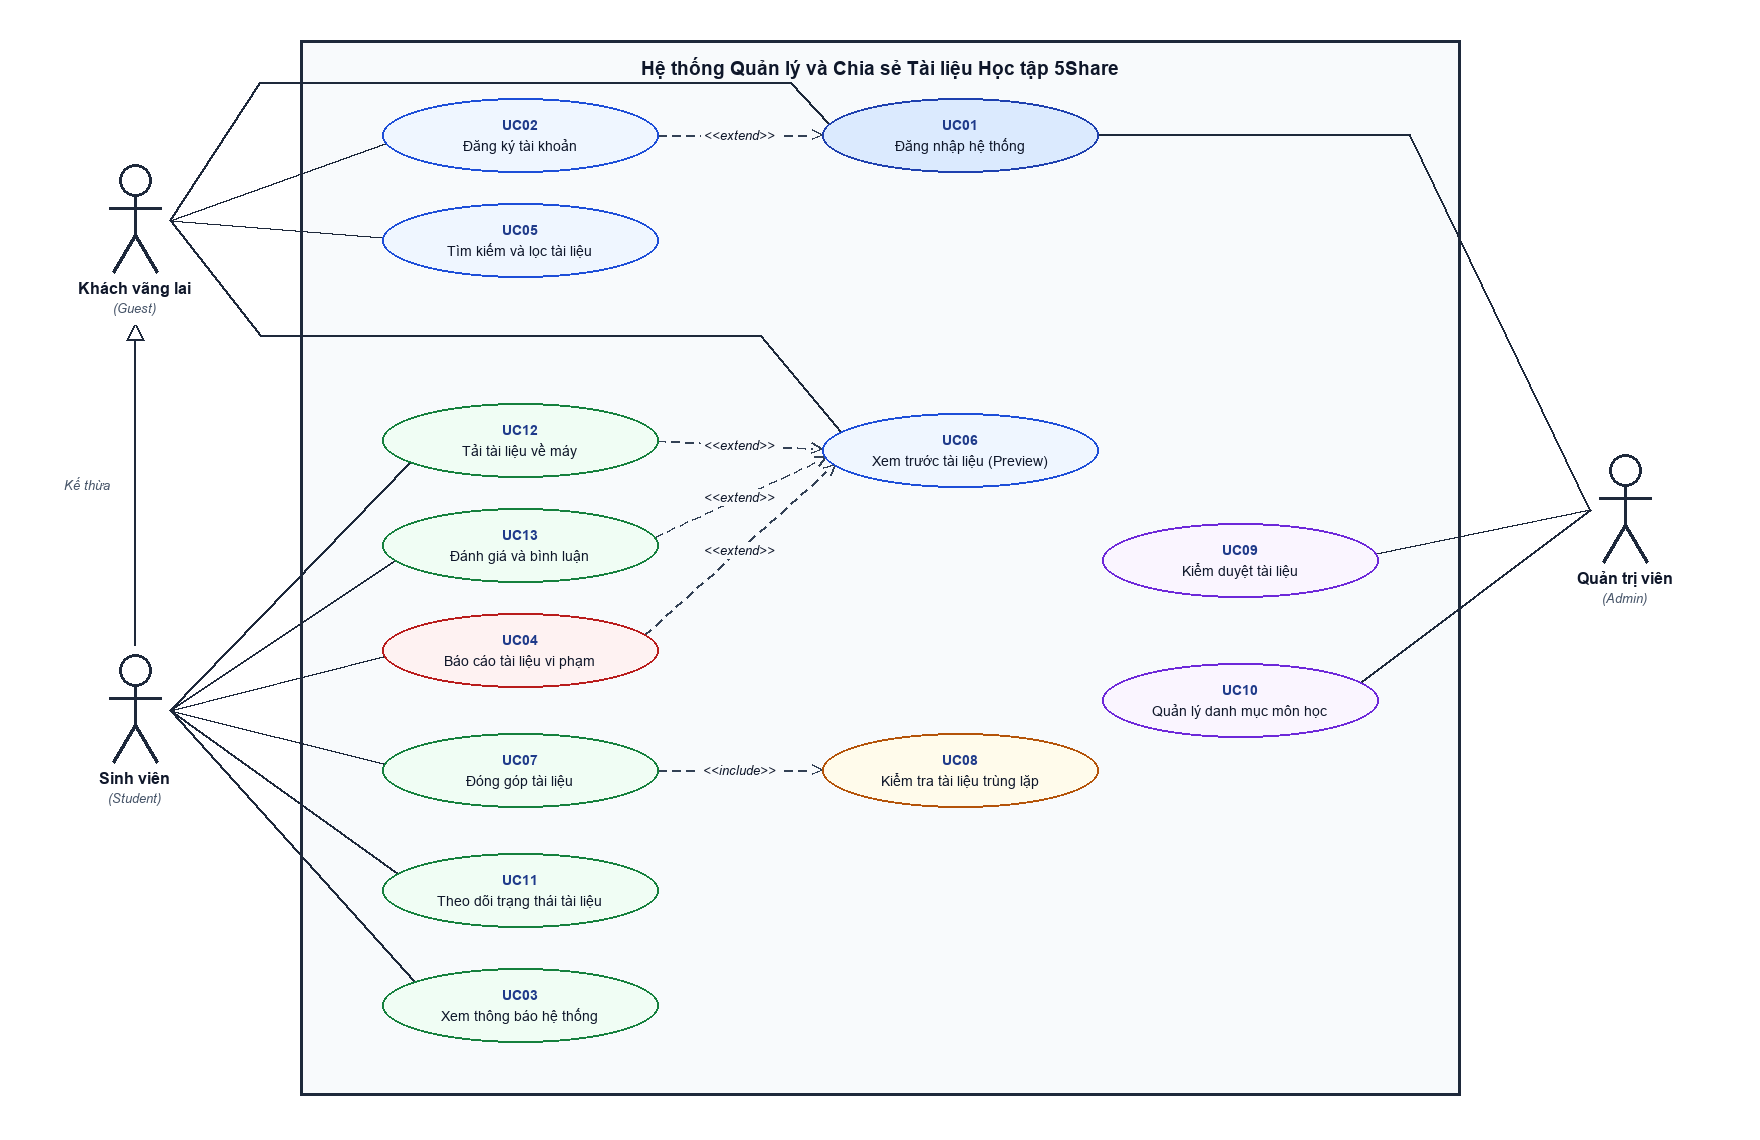
\includegraphics[width=0.98\textwidth]{chuong2/images/so_do_use_case_tong_quan.png}%
}{%
    \fbox{\parbox{0.95\textwidth}{\centering \vspace{3cm}\textbf{[Hình 2.1: Biểu đồ Use Case tổng quan của hệ thống 5Share]}\vspace{3cm}}}%
}
\caption{Biểu đồ Use Case tổng quan của hệ thống 5Share}
\label{fig:uc_tong_quan}
\end{figure}

\subsubsection{2.2.2. Biểu đồ Use Case phân rã cụm chức năng xác thực}
Để làm rõ các luồng mở rộng và cơ chế kiểm tra phân quyền tự động trong quá trình xác thực người dùng, ca sử dụng \texttt{UC01} (Đăng nhập hệ thống) được phân rã chi tiết ở mức 2 như minh họa tại Hình~\ref{fig:uc01_phan_ra}. Trong đó, ca sử dụng đăng nhập luôn bao hàm (\texttt{<<include>>}) bước xác thực mã phiên JWT và phân quyền theo vai trò lưu trong cơ sở dữ liệu, đồng thời cho phép mở rộng (\texttt{<<extend>>}) sang đăng ký tài khoản mới (\texttt{UC02}), khôi phục mật khẩu hoặc đăng nhập nhanh qua giao thức Google OAuth 2.0.

\begin{figure}[H]
\centering
\IfFileExists{chuong2/images/so_do_uc01_dang_nhap.png}{%
    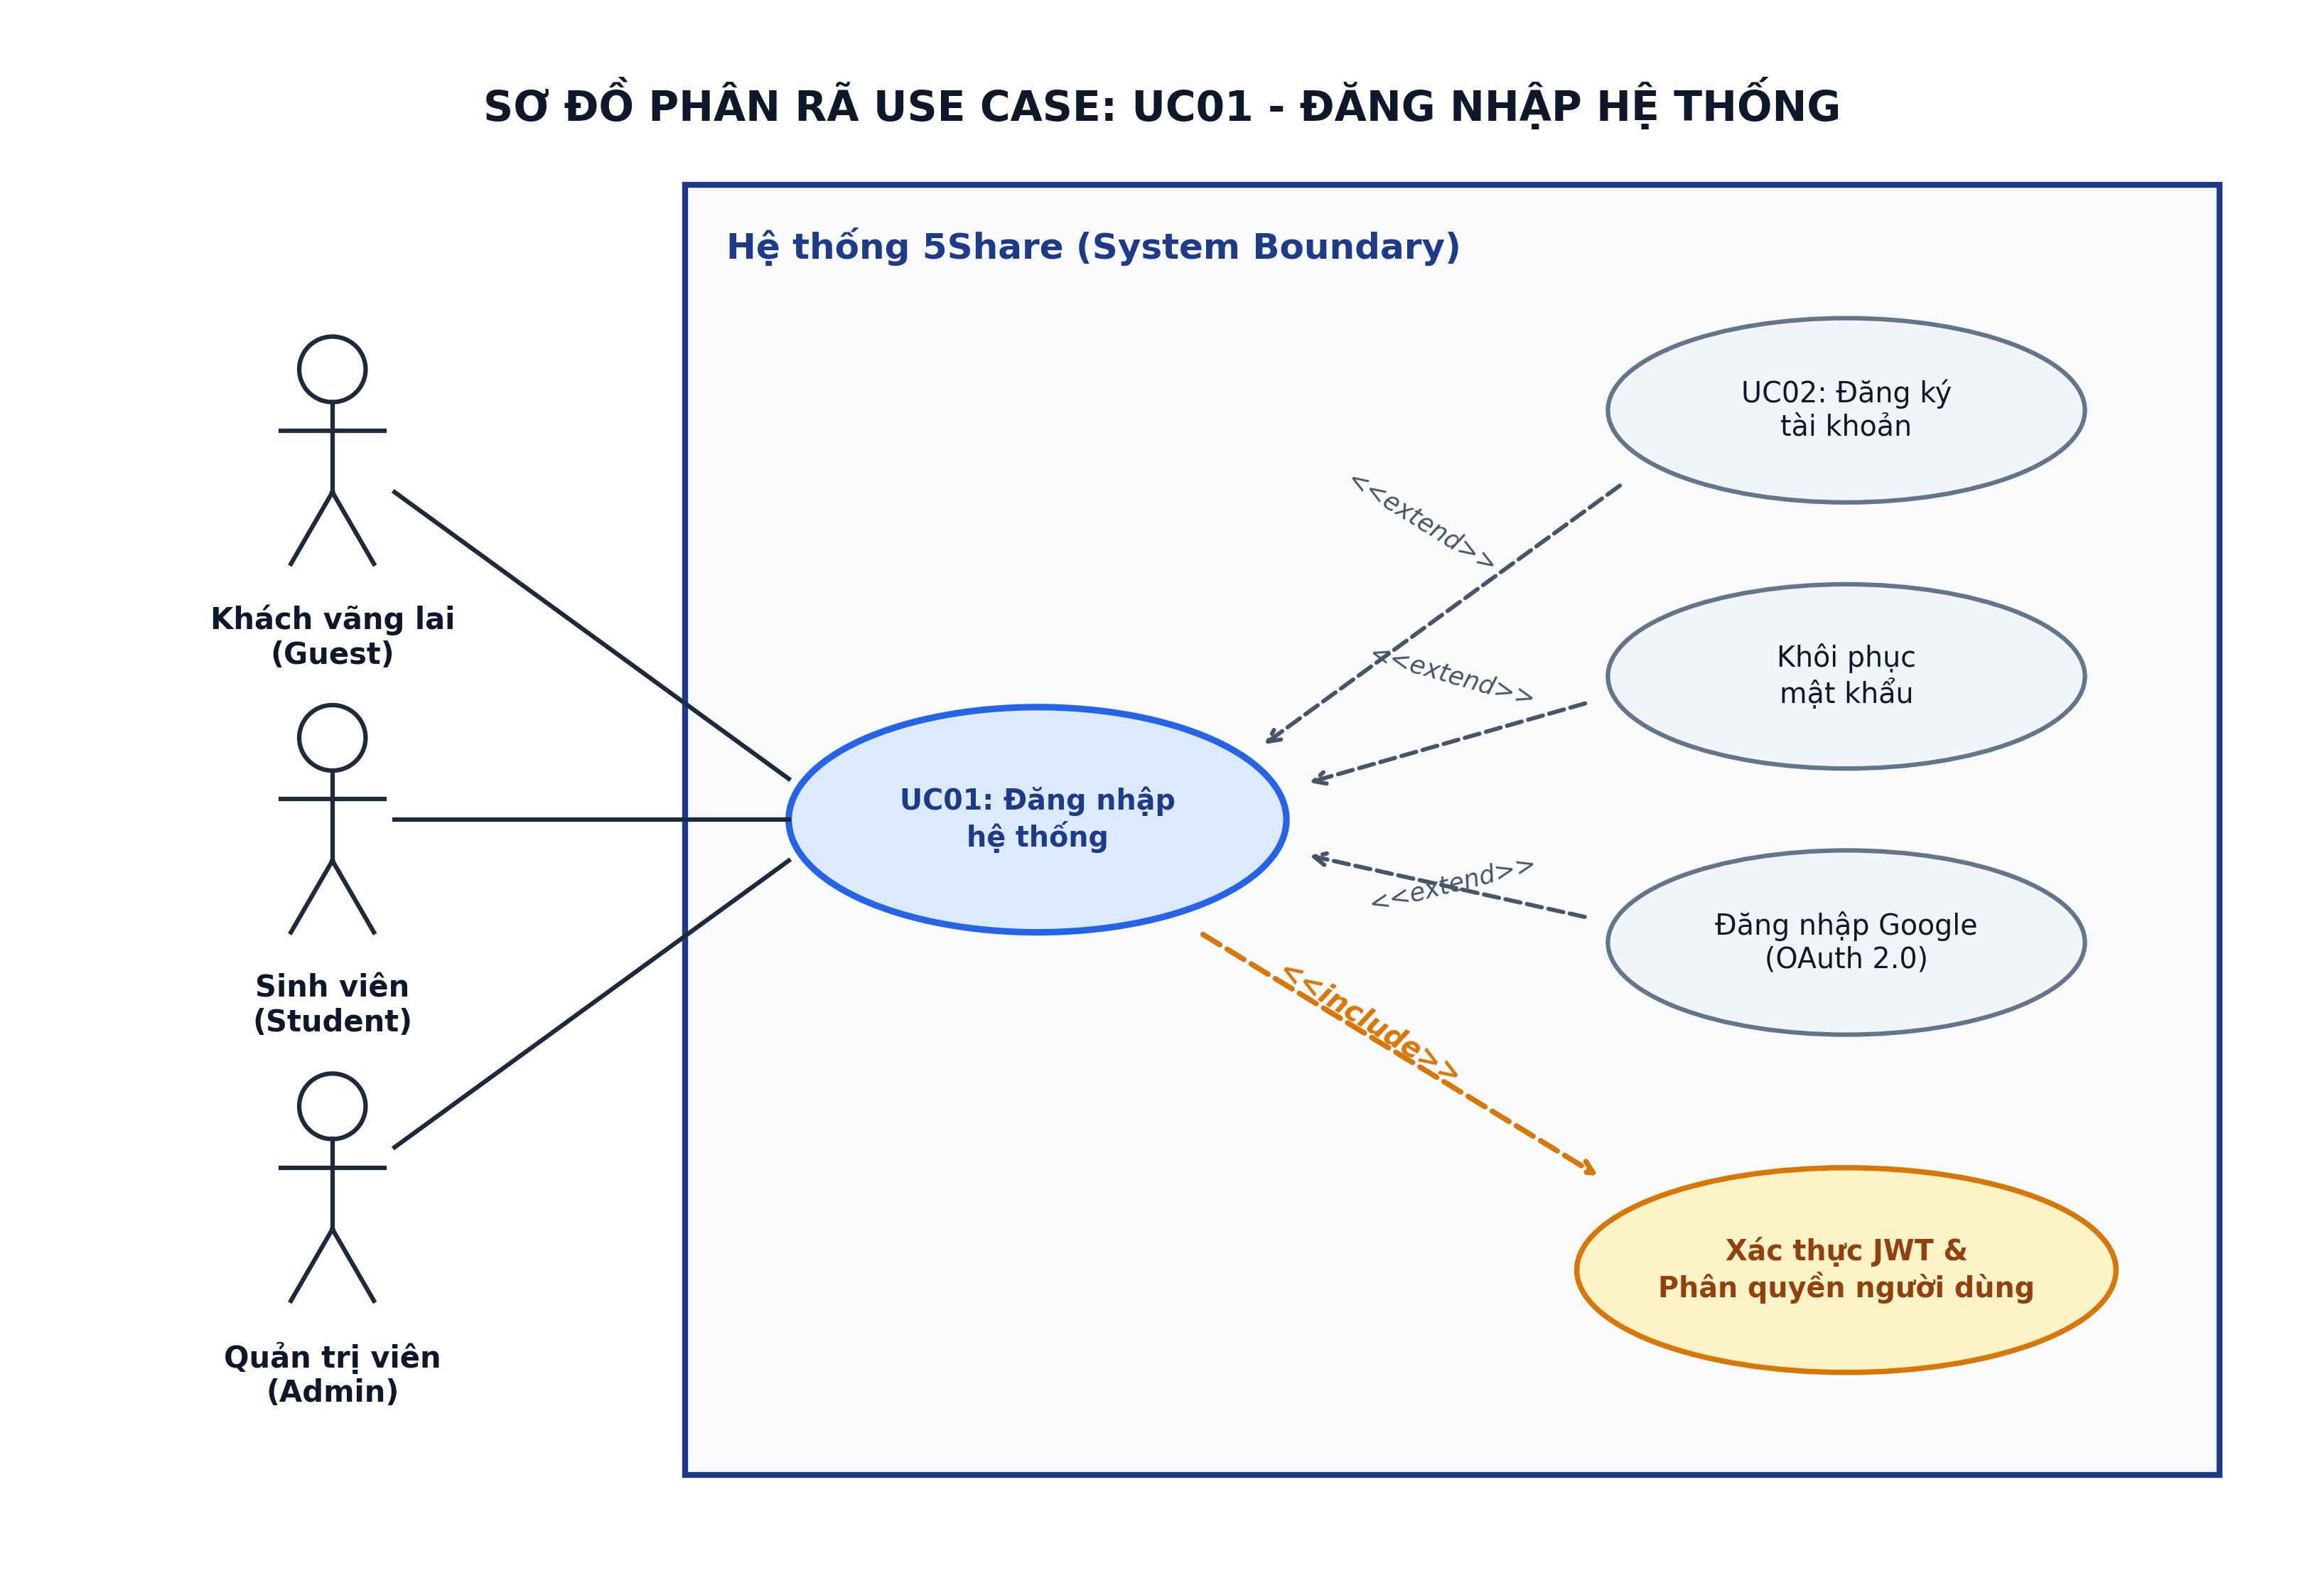
\includegraphics[width=0.92\textwidth]{chuong2/images/so_do_uc01_dang_nhap.png}%
}{%
    \fbox{\parbox{0.95\textwidth}{\centering \vspace{3cm}\textbf{[Hình 2.2: Biểu đồ Use Case phân rã chi tiết ca sử dụng Đăng nhập hệ thống (UC01)]}\vspace{3cm}}}%
}
\caption{Biểu đồ Use Case phân rã chi tiết ca sử dụng Đăng nhập hệ thống (UC01)}
\label{fig:uc01_phan_ra}
\end{figure}
